\section{}



\subsection{}

Wir plotten \texttt{L} durch den folgenden zusätzlichen Code:

\lstinputlisting[style=pythoncode, firstline = 21, lastline = 29]{chapter_04/exercise_04_23.py}

Wir erhalten hierdurch das folgende Bild:

\begin{center}
  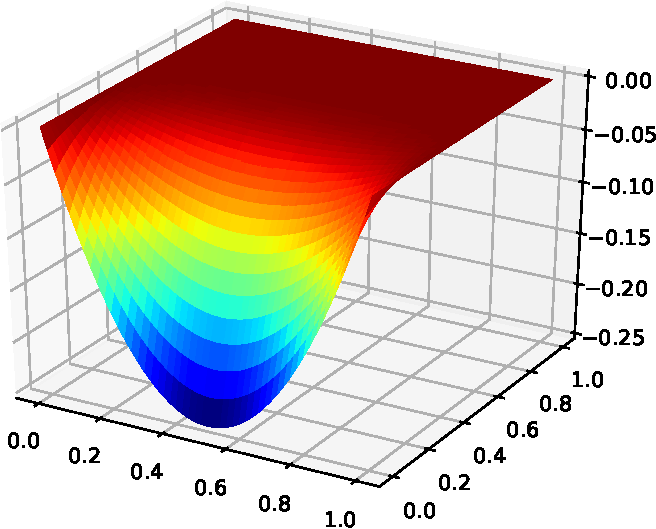
\includegraphics[width = 0.8\textwidth]{chapter_04/exercise_04_23_figure_1.pdf}
\end{center}



\subsection{}

Das Programm berechnet für $\Omega = (0,1) \times (0,1)$ eine approximative Lösung der Differentialgleichung
\begin{gather*}
  \text{$\Delta u = 0$ auf $\Omega$}
  \qquad\text{und}\qquad
  \text{$u = g$ auf $\partial \Omega$}.
\shortintertext{wobei}
    g(x,y)
  = \begin{cases}
      y(y-1)  & \text{falls $x = 0$},  \\
      0       & \text{sonst}.
    \end{cases}
\end{gather*}
Dabei soll für alle für alle $i,j = 0, \dotsc, 50$ der Eintrag \texttt{L[i,j]} approximativ dem Funktionswert $u(i/50, j/50) \eqqcolon u_{ij}$ entsprechen.
Die aus
\[
  \text{$u = g$ auf $\partial \Omega$}
\]
folgenden Randbedingungen werden durch die folgende Zeile des Codes festgelegt:
\lstinputlisting[style=pythoncode, firstline = 8, lastline = 8]{chapter_04/exercise_04_23.py}
Man bemerke, dass die Randwerte \texttt{L[i,j]} (mit $i = 0, 50$ und $j = 0, 50$) im Laufe des Programmes unverändert bleiben.
Die Gleichung
\[
  \text{$\Delta u = 0$ auf $\Omega$}
\]
wird mit
\[
    \frac{1}{h^2} ( - u_{i-1,j} - u_{i,j-1} + 4 u_{ij} - u_{i+1,j} - u_{i,j+1} )
  = f(ih, jh)
  \overset{!}{=} 0
\]
(siehe Abschnitt 4.8, Seite 60 im Skript) durch die folgende Gleichung des Codes implementiert:
\lstinputlisting[style=pythoncode, firstline = 15, lastline = 15]{chapter_04/exercise_04_23.py}

Der Code funktioniert also dadurch, dass auf dem Rand mit den exakten Werten für $u_{ij}$ begonnen wird, und diese dann mithilfe der Gleichung
\[
    u_{ij}
  = \frac{u_{i-1,j} + u_{i,j-1} + u_{i+1,j} + u_{i,j+1}}{4}
\]
auch nach innen hin propagiert werden.

Um unsere Vermutung zu überprüfen, bestimen wir mithilfe der gegebenen Methode \texttt{poisson\_solver} die exakte Lösung, und plotten diese:

\lstinputlisting[style=pythoncode, firstline = 33, lastline = 39]{chapter_04/exercise_04_23.py}

Wir erhalten den folgenden Graphen:

\begin{center}
  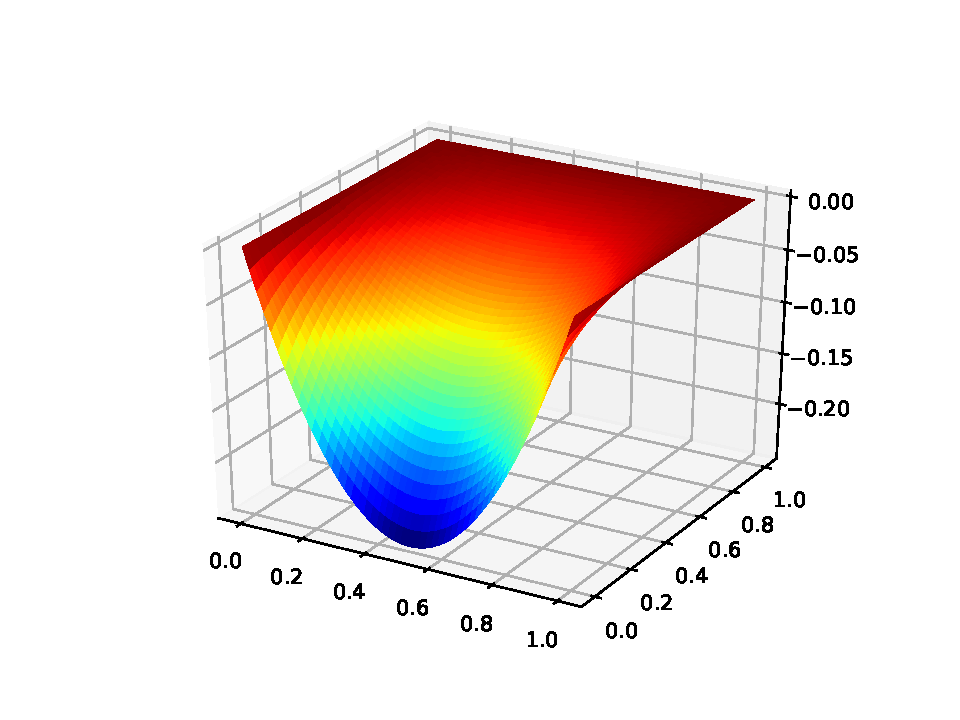
\includegraphics[width = 0.8\textwidth]{chapter_04/exercise_04_23_figure_2.pdf}
\end{center}

Der Vergleich mit dem obigen Graphen bestätigt unsere Vermutung.
